%%%%%%%%%%%%%%%%%%%%%%%%%%%%%%%%%%%%%%%%%%%%%%%%%%%%%%%%%%%%%%%%%%%%%%%%%%%%%%%%%
% Author: First Name Last Name
% Type: Semester/Master Thesis
% Title: Thesis Title
%%%%%%%%%%%%%%%%%%%%%%%%%%%%%%%%%%%%%%%%%%%%%%%%%%%%%%%%%%%%%%%%%%%%%%%%%%%%%%%%%

\documentclass[pdflatex,11pt,a4paper,twoside,titlepage]{scrbook}

%---------packages------------------------------------------------------

\usepackage[english]{babel}
\usepackage[latin1]{inputenc}
\usepackage{a4wide}

\usepackage{amsmath}
\usepackage{amsfonts}
\usepackage{amssymb}
\usepackage{mathcomp}

%\addtokomafont{disposition}{\rmfamily}				% uncomment for serif fonts for headings KOMA classes
\usepackage[hang,labelfont=bf]{caption}				% configure captions of images, tables etc.
%\usepackage[footnotesize,sl,SL,hang,tight]{subfigure}		% helpful package for aligning figures next to each other
%\usepackage{captcont}						% continue sufigures over several pages

\usepackage{verbatim}
\usepackage{booktabs}							% publication quality tables for LaTeX
%\usepackage{multirow}						% cells in tables can span multiple rows
%\usepackage{rotating}
\usepackage{fancyhdr}

\usepackage[pdftex]{color,graphicx}
%\usepackage[hang]{caption}
\usepackage{subfigure}
\usepackage{color}
\usepackage{float}
\usepackage{hyperref}
\usepackage{listings}
\lstset{keywordstyle=\color{blue}\bfseries\emph, breaklines=true, breakatwhitespace=false}
\lstset{language=C, basicstyle=\footnotesize, commentstyle=\color{green}}
\hypersetup
{
pdftitle = {Thesis Title},
pdfauthor = {Name},
colorlinks = {true},
hypertexnames={true},
plainpages={false},
linkcolor={black},
citecolor={black},
filecolor={black},
urlcolor={black},
anchorcolor={black},
menucolor={black},
breaklinks={true}
}

%\setlength{\textwidth}{15cm}
%\setlength{\textheight}{22.0cm}
%\setlength{\oddsidemargin}{0.75cm}
%\setlength{\evensidemargin}{-0.3cm}
%\setlength{\topmargin}{-0.2cm}			% Distance between page top and header
\setlength{\headheight}{15pt}
%\setlength{\parskip}{1.5explus0.5ex}
%\setlength{\parindent}{0pt}				% \noindent
%\renewcommand{\baselinestretch}{1.2}		% Line distance
%\setcounter{secnumdepth}{3}			% Displays Section number down to 3 ranks
%\setcounter{tocdepth}{3}

\newcommand{\clearemptydoublepage}{\newpage{\pagestyle{empty}\cleardoublepage}}
\newcommand{\st}{\stackrel{*}}

%---------document------------------------------------------------------

\begin{document}

\frontmatter

\thispagestyle{empty}
\enlargethispage{2cm} 

\begin{center}
		\vspace*{-3.3cm}
    \rule{\linewidth}{0.5pt} \\
\end{center}


\includegraphics[width=.4\textwidth]{ethlogo}
\vspace{-1.2cm} 

\begin{center}
		\vspace*{0.4cm}
    \rule{\linewidth}{0.5pt} \\
\end{center}


\begin{center}
  \vspace*{.8cm}
  \LARGE \bfseries \boldmath
 Thesis Title
  \vspace*{0.5cm} \unboldmath
\end{center}


\begin{figure}[htb!]
	\centering
  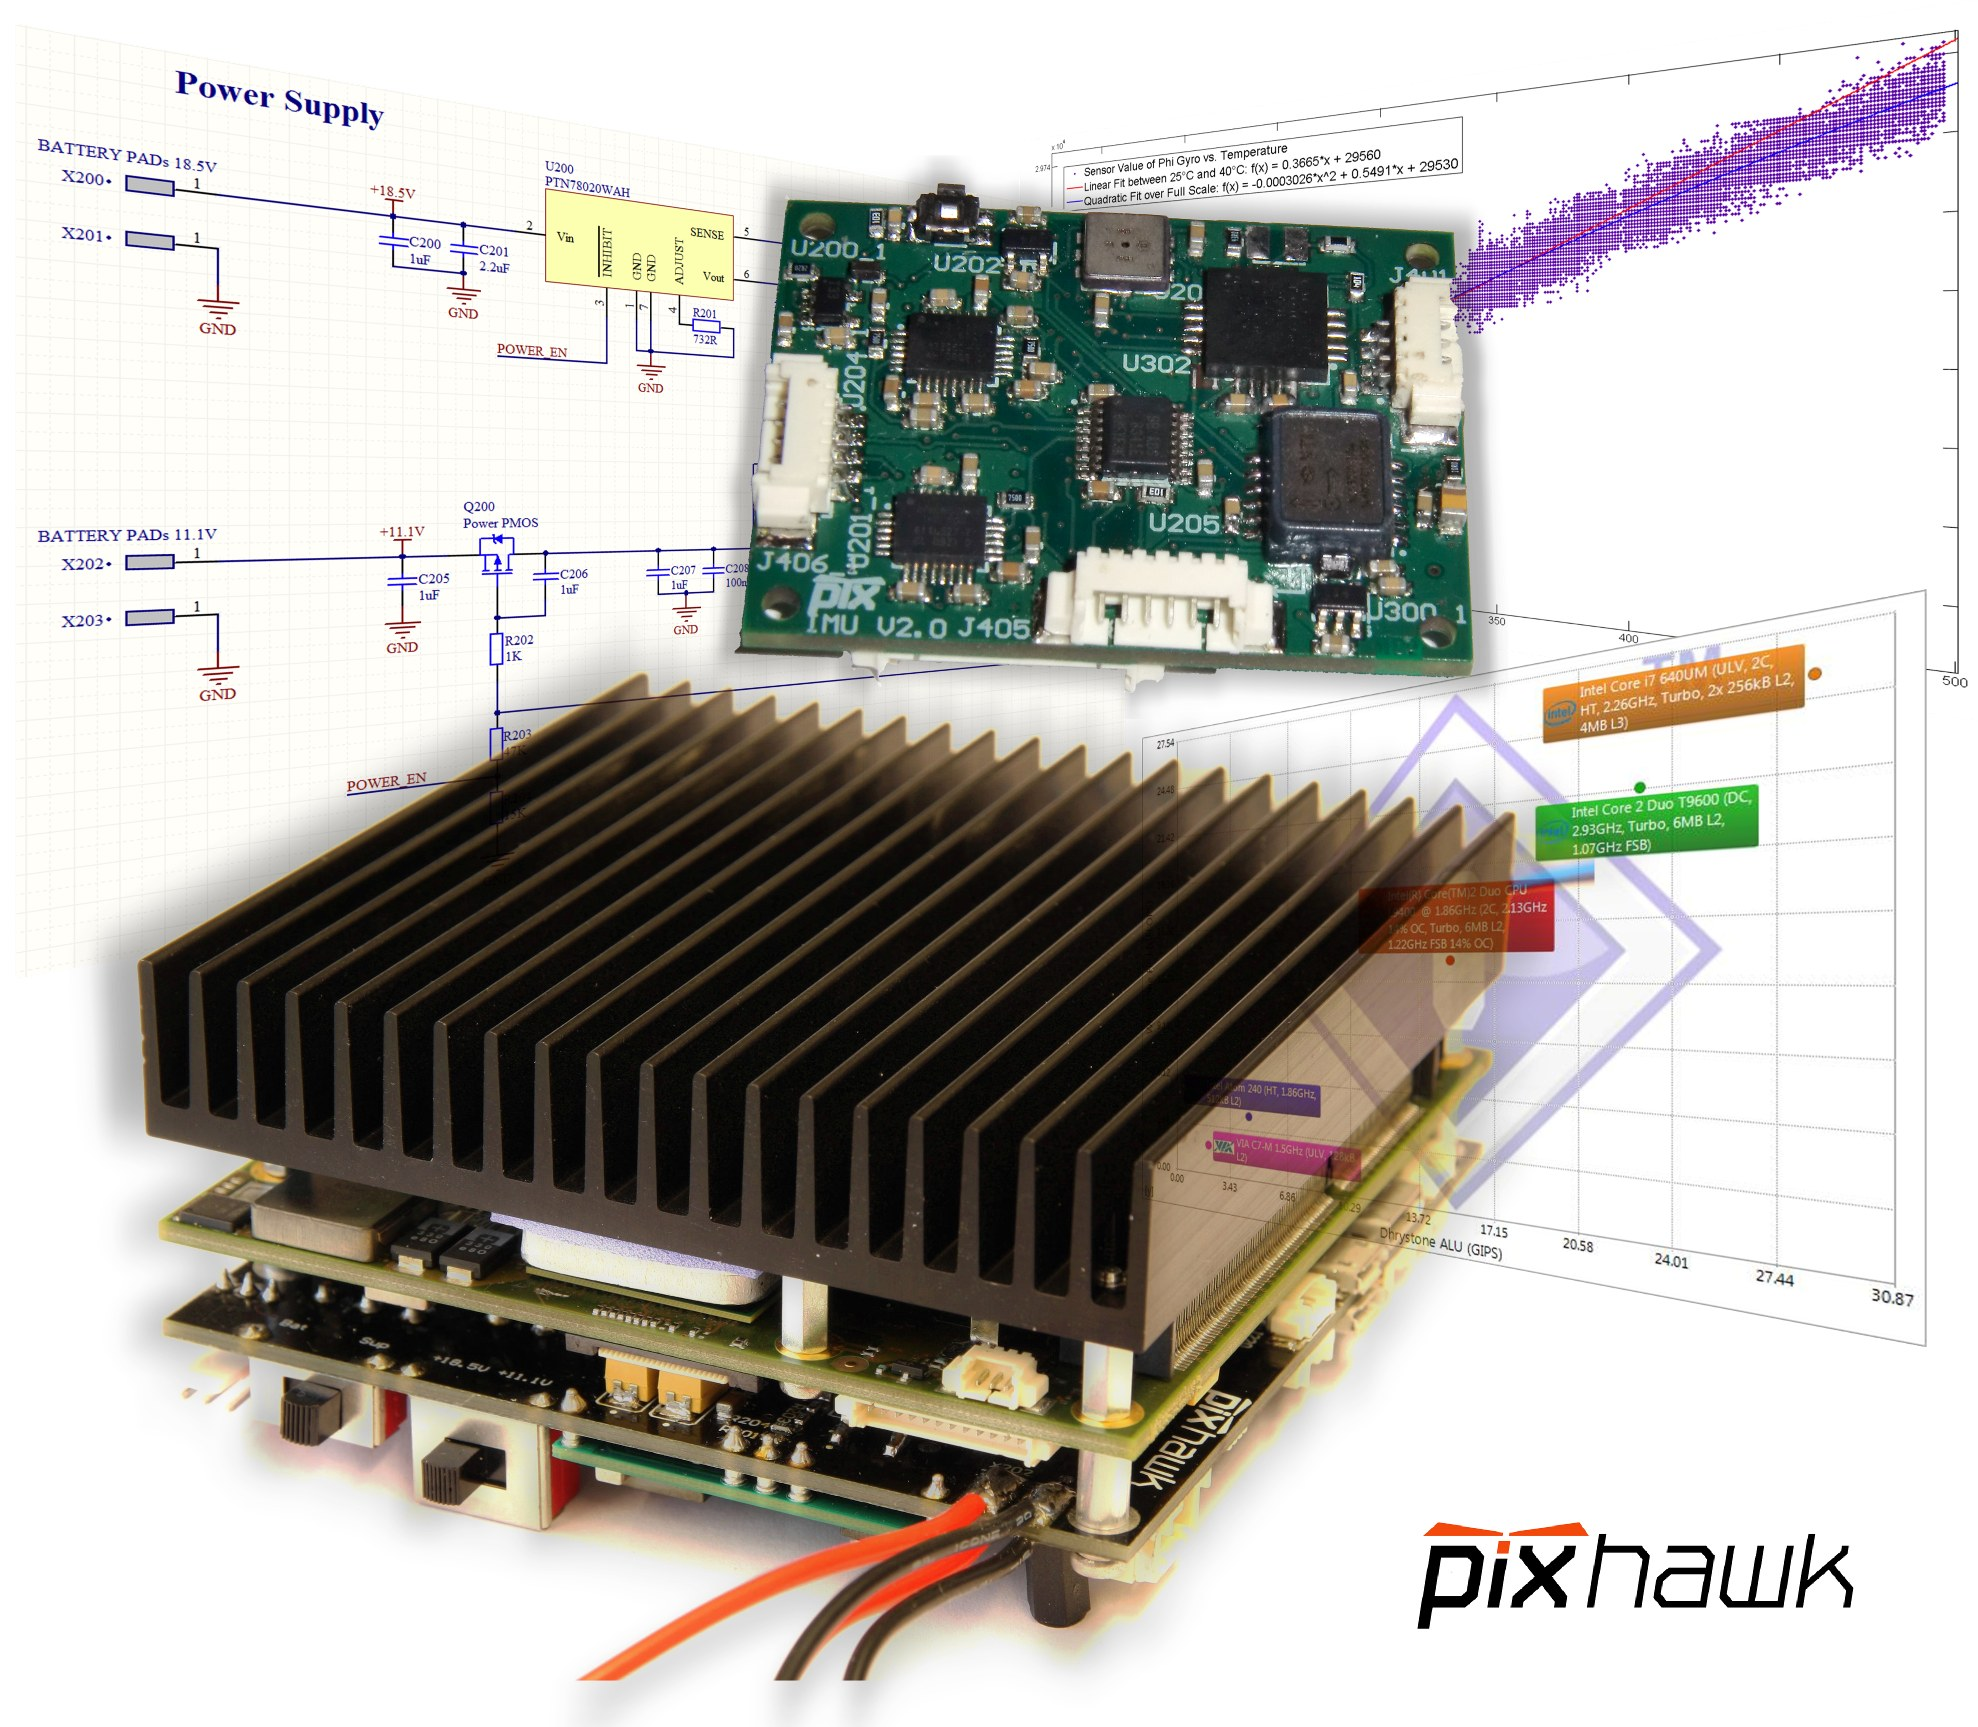
\includegraphics[width=0.9\textwidth]{titlepageimage.jpg}\\
\end{figure}

\begin{center}
  \vspace*{0.5cm}
  \Large
  \textit{Master Thesis CVG Lab\\SS 2017} \\
  \vspace{1cm}
  \Large \mdseries
  Daniel Keyes\\
  \vspace{0.5cm}
\end{center}

\begin{center}
    \rule{\linewidth}{0.5pt} \\
\end{center}

\Large

\begin{tabular}{l@{\hspace{0.5cm}}l}
  Advisors: 	& Federico Camposeco\\
  Professor: 	& Prof. Marc Pollefeys
\end{tabular}

\normalfont \normalsize

\clearemptydoublepage
\chapter{Abstract}

In any camera motion estimation pipeline, the problem of relocalization---determining where a camera is located in a previously constructed map---must be addressed to recover from tracking loss, minimize drift, and remain reliable over time. Whereas traditionally these maps have contained only a very sparse cloud of points, recent developments in visual odometry have shown that it is possible to generate a relatively dense point cloud while tracking camera motion. In this work, we leverage this rich geometric information to perform camera relocalization. We adopt approaches that were previously viable only with dedicated depth-sensing hardware; we analyze our results on two well-known relocalization benchmarks; and we analyze failure cases.

\clearemptydoublepage
\chapter{Acknowledgments}

Acknowledgments to people who supported you. In Semester theses this chapter can be removed.

\clearemptydoublepage

%list of contents, figures and tables
\phantomsection
\addcontentsline{toc}{chapter}{Contents}
\tableofcontents
\cleardoublepage
\phantomsection
\addcontentsline{toc}{chapter}{List of Figures}
\listoffigures
\cleardoublepage
\phantomsection
\addcontentsline{toc}{chapter}{List of Tables}
\listoftables
\cleardoublepage

%customize headers and footers
\pagestyle{fancyplain} % Chapter and Section appear in header
\renewcommand{\chaptermark}[1]{\markboth{#1}{}} % Changes chapter appearence
\renewcommand{\sectionmark}[1]{\markright{\thesection\ #1}} % Changes section appearence
\lhead[\fancyplain{}{\bfseries\thepage}]{\fancyplain{}{\bfseries\rightmark}}
\rhead[\fancyplain{}{\bfseries\leftmark}]{\fancyplain{}{\bfseries\thepage}}
%\cfoot{} % removes page number from footer
\cfoot[\fancyplain{}{}]{\fancyplain{\thepage}{}} %Page number in the first page of a chapter in footer 

%--------- include chapters----------------------------------------------
\mainmatter

\graphicspath{{chapter1/}}

\chapter{Chapter1}
\label{cha:chapter1}

This is the first chapter of the template thesis of the PIXHAWK project.\\

\begin{figure}[htbp]
	\centering
		
\includegraphics[width=0.60\textwidth]{pixhawk-logo.png}
	\caption{The PIXHAWK project logo \cite{pix_wiki}}
	\label{fig:pixhawk-logo}
\end{figure}

\section{The PIXHAWK Project}
\label{sec:pixhawkproject}

PIXHAWK is a student project team of the Computer Vision and Geometry (CVG) Lab at the ETH Zurich. The goal of the PIXHAWK project is to build a helicopter that will be able to explore indoor and outdoor environments autonomously and identify objects or classes of objects. Typical usage scenarios are visual inspection of air conditioning systems, and disaster recovery. In disaster recovery, the helicopter will enter semi-collapsed buildings and search for victims needing assistance. Due to the small size and the non-surface-touching drive mechanism, the helicopter can enter locations not accessible by ground robots, dogs or humans.

\cleardoublepage

\chapter{Chapter 2}

This is Chapter 2 with some math.

\begin{equation}
\label{eq:some_equation}
\mathbf{x'}_i \times \texttt{H}\mathbf{x}_i = 
\begin{bmatrix}
\mathbf{0}^{\top} & -w'_i\mathbf{x}_i^{\top} & y'_i\mathbf{x}_i^{\top} \\
w'_i\mathbf{x}_i^{\top} & \mathbf{0}^{\top} & -x'_i\mathbf{x}_i^{\top} \\
-y'_i\mathbf{x}_i^{\top} & x'_i\mathbf{x}_i^{\top} & \mathbf{0}^{\top} \\
\end{bmatrix}
\begin{pmatrix}
\mathbf{h}^{1} \\ 
\mathbf{h}^{2} \\ 
\mathbf{h}^{3}
\end{pmatrix}
= \mathbf{0}
\end{equation}

It can be also included directly in to the text $x = y$.

And some tables (\ref{tab:some_table}) too.

\begin{table}[!h]
\begin{center}
\begin{tabular}{c c c c c c c c}
\toprule
Sample size & \multicolumn{7}{c}{Proportion of outliers $\epsilon$}\\
\midrule
s & 5\% & 10\% & 20\% & 25\% & 30\% & 40\% & 50\% \\
\midrule
2 & 2 & 3 & 5 & 6 & 7 & 11 & 17 \\
3 & 3 & 4 & 7 & 9 & 11 & 19 & 35 \\
4 & 3 & 5 & 9 & 13 & 17 & 34 & 72 \\
5 & 4 & 6 & 12 & 17 & 26 & 57 & 146 \\
6 & 4 & 7 & 16 & 24 & 37 & 97 & 293 \\
7 & 4 & 8 & 20 & 33 & 54 & 163 & 588 \\
8 & 5 & 9 & 26 & 44 & 78 & 272 & 1177 \\
\bottomrule
\end{tabular}
\end{center}
\caption[Required samples for RANSAC]{The number $N$ of samples required to ensure, with a probabilty $p = 0.99$, that at least one sample has no outliers for a given size of sample $s$, and proportion of outliers $\epsilon$.}
\label{tab:some_table}
\end{table}

\backmatter

%Bibliography
%\bibliographystyle{IEEEtran}		% use this for electric engineering thesis (contains support for datasheets)
\bibliographystyle{splncs}		% use this for computer vision thesis
\bibliography{thesis}
\cleardoublepage

%\appendix
%\include{appendix/appendix}

\end{document}
